\section{Systematics Uncertainties in the Background Prediction}
\label{sec:systematics}

We discuss here the sources of uncertainty in the background predictions from the MET templates and OF subtraction methods.

\subsection{Template Method Related Systematics}
In this section, we list several sources of systematic uncertainties related to the template method,
as summarized in Table.~\ref{tab:templatesyst}. We perform several variations in the template prediction,
and check the corresponding relative difference in the predicted yield for the loose signal region.
We have checked that the variations in the predicted yield do not depend strongly on the MET cut,
within statistical uncertainties. 

\begin{table}[hbt]
\begin{center}
\caption{\label{tab:templatesyst} Summary of variations in the MET templates prediction. The yields predicted
by the MET templates method in the loose signal region (MET$>60$ GeV) are shown, along with the 
relative difference with respect to the nominal prediction, for several sources of variation in the 
template prediction.}
\begin{tabular}{l|cc}
\hline
                                      & N(MET$>60$ GeV)   & Rel Diff    \\%&  N(MET$>120$ GeV)    & Rel Diff      \\  
\hline
Nominal                               & 1.81 $\pm$ 0.13   &             \\%&   0.14  $\pm$  0.03  &               \\
nVtx reweighting                      & 1.79 $\pm$ 0.13   & -0.01       \\%&   0.14  $\pm$  0.03  &    0.00       \\
hadronic recoil $P_T$ reweighting     & 2.27 $\pm$ 0.21   & +0.25       \\%&   0.17  $\pm$  0.04  &   +0.21       \\
vary photon selection (emf $>0.8$)    & 1.73 $\pm$ 0.17   & -0.04       \\%&   0.20  $\pm$  0.06  &   +0.42       \\
vary photon selection (emf $>0.9$)    & 2.27 $\pm$ 0.35   & +0.25       \\%&   0.31  $\pm$  0.13  &   +1.21       \\
vary photon selection (h/e $<0.05$)   & 1.52 $\pm$ 0.12   & -0.16       \\%&   0.11  $\pm$  0.03  &   -0.21       \\
vary photon selection (h/e $<0.01$)   & 2.18 $\pm$ 0.37   & +0.20       \\%$   0.24  $\pm$  0.12  &   +0.71       \\
\hline
\end{tabular}
\end{center}
\end{table}


\begin{itemize}
\item A difference in \Z \pt vs photon \pt introduces a difference in the boost of the hadronic system,
  which affects the MET distribution due to coherent mismeasurement of the hadronic activity. 
  We test this using a reweighting procedure based on the distribution of the hadronic recoil $P_T$ 
  in the \Z and photon samples. We normalize to unit area the distributions of hadronic recoil \pt in the 2 samples,
  and assess to each photon event a weight which is equal to the ratio of the \Z:\pt contributions in the corresponding
  bin of hadronic recoil \pt. This procedure gives a relative difference of 25\% in the predicted yield and
  we assess a corresponding uncertainty.
\item The photon triggers are prescaled as the instantaneous luminosity increased. As a result, the 
  number of pile up events is different in \Z events than in photon events, 
  as the latter were preferentially taken at lower instantaneous luminosity. However, this difference
  is largely compensated because the photon events are weighted by the trigger rescale. We perform the
  same reweighting procedure using the nVertex distribution in \Z and photon events. This procedure gives
  uncertainties of less than 1\%, which we regard as negligible.
\item Backgrounds to the photon sample from events where the ``photon object'' includes 
  hadronic energy that was lost will artificially increase the MET templates. 
  If this was a significant effect, then  altering the photon selection ought to significantly 
  change the MET prediction. We test for this
  by by tightening the cuts on neutral EM fraction and
  h/e. Based on these studies we assess an uncertainty of 25\% 
  %{\bf Not sure how much uncertainty to assess here.
  %Going to h/e $<$ 0.01 and emf $>$ 0.9 change the prediction by 25\% and 21\% but the stat uncertainty is large.
  %Something like 30\% seems reasonable (but conservative)...}

%\item {\bf Need to add MC closure here}

\end{itemize}

Based on these studies we assess an uncertainty of 25\% 
%{\bf Will update this after decided on syst for
%photon selection and MC closure }
on the MET templates background prediction,
which is entirely dominated by the difference in the \Z vs. photon hadronic recoil \pt distributions. We therefore 
predict the following Z + jets + MET background predictions using the MET templates method: \\
loose signal region:  1.81 $\pm$ 0.13 (stat) $\pm$ 0.45 (syst) \\
tight signal region:  0.14 $\pm$ 0.03 (stat) $\pm$ 0.04 (syst).

%Any residual lepton mismeasurement effects are tested for by varying the \Z mass window. [PLOT?]

\subsection{Systematics of OF Subtraction}
\label{sec:systematicsof}

The uncertainty on the background prediction from the OF subtraction comes from the uncertainties in 2
quantities: $\epsilon_{e\mu} = \epsilon(e)/\epsilon(\mu)$, the ratio of muon to electron selection efficiencies,
and $K$, the fraction of $t\bar{t}$ events which fall inside the \Z mass window.
The uncertainty in $\epsilon_{e\mu}$ is due to the fact that the efficiencies are measured in a \Z sample and applied to
a $t\bar{t}$ sample. In the ttdilepton cross-section measurement the isolation efficiencies are found to
vary by 4\% per lepton in \Z vs. $t\bar{t}$ events. We therefore assess a 5\% uncertainty in $\epsilon_{e\mu}$, which
is conservative because the difference in isolation efficiency is due to an increase in hadronic activity
which is modeled in the MC, and also because $\epsilon_{e\mu}$ is a ratio and the uncertainty partially cancels.
The uncertainty in $K$ is due to the uncertainty in the lepton energy scale and is therefore quite small.
Varying the boundaries of the \Z mass window by $\pm2$~GeV results in a relative change in $K$ of 2\% 
and we assess a corresponding uncertainty.

Based on these studies we find the following predicted $t\bar{t}$ yields from the OF subtraction technique: \\
loose signal region:  4.24 $\pm$ 0.82 (stat) $\pm$ 0.23 (syst)  \\
tight signal region:  1.10 $\pm$ 0.42 (stat) $\pm$ 0.06 (syst).




%%%-----------------------------------------------------------------------------------------------------------
%This is a search for new physics contributions to 
%\Z events with high \met and jet activity.
%As seen in Section~\ref{sec:results}, there is no
%evidence for a contributions beyond SM expectations.

%Strictly speaking it is impossible to talk about 
%``acceptance systematics'' because these kinds of
%systematics only apply to a well defined final state.
%Nevertheless, we can at least make some qualitative
%statements.

%The systematic uncertainty on the lepton acceptance consists
%of two parts: the trigger efficiency uncertainty and the 
%ID and isolation uncertainty.  We discuss these in turn.
%
%The trigger efficiency 
%for two leptons of \pt $> 20$ GeV is very high, except in some corners
%of phase space (see Section~\ref{sec:trgEff}).  
%We estimate the efficiency uncertainty to be a few percent.%, mostly in the low \pt region.

%\begin{figure}[tbh]
%\begin{center}
%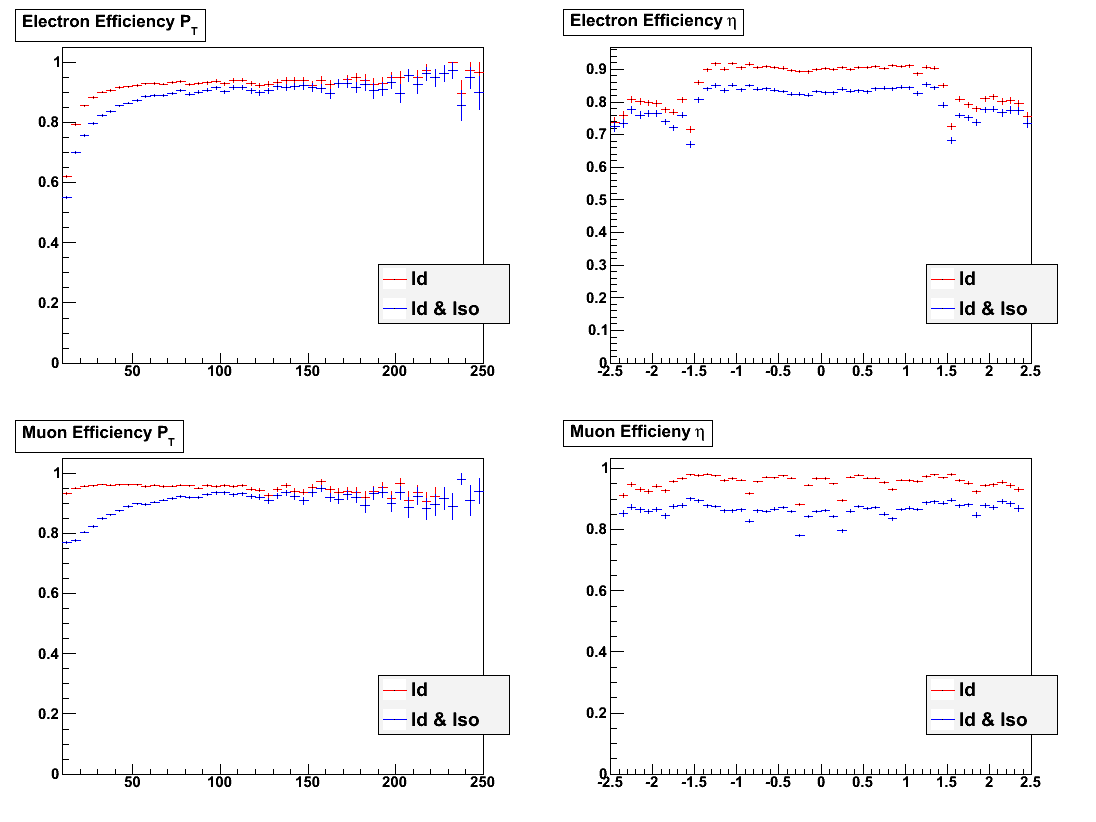
\includegraphics[width=0.75\linewidth]{plots/eff_11.png}
%\caption{\label{fig:effttbar}\protect 
%Identification and isolation efficiencies for 
%leptons from $t \to W \to \ell$ and 
%$t \to W \to \tau \to \ell$ in 
%$t\bar{t}$ events.}
%\end{center}
%\end{figure}


%The ID efficiencies in MC are shown in 
%Figures~\ref{fig:effttbar}
%for the leptons from $t \to W \to \ell$ and $t \to W \to \tau \to \ell$.
%Tag and probe studies show that these are correct to about 
%{\bf xx\%.  (We need to do tag-and-probe on the full sample,
%see what we get, and write text accordingly).}

%The isolation efficiency depends on the jet activity in
%the final state.  For example, in MC we find that the
%lepton isolation efficiency differs by $\approx 4\%$ 
%{\bf per lepton} between $Z$ events and $t\bar{t}$ events\cite{ref:top}\cite{ref:toptwiki}.

%Another significant source of systematic uncertainty is 
%associated with the jet and $\met$ energy scale.  The impact
%of this uncertainty is very final state dependent.  Final
%states characterized by lots of hadronic activity and \met are much
%less sensitive than final states where the \met and sum jet \pt
%are typically close to the requirement.  To be more quantitative,
%we have used the method of Reference~\cite{ref:top} to evaluate
%the systematic uncertainties on the acceptance for $t\bar{t}$ 
%and two benchmark SUSY points.  The uncertainties are calculated
%assuming a 5\% uncertainty to the hadronic energy scale in CMS.

%{\bf For $t\bar{t}$ we find uncertainties of xx\% (baseline 
%selection) and yy\% (signal region D); for LM0 and LM1 we find
%xx\% and yy\% respectively for signal region D.}

%%%-----------------------------------------------------------------------------------------------------------

















%[?] Systematics are derived using three methods: varying Njet threshold, varying photon pt requirement for templates, and cutting on the pt of the Z.

%
%\subsection{Pile Up related}
%\label{sec:pileupsyst}
%Events in the pp collision data sample have, on average, slightly above one extra pp collision in the same 
%bunch crossing. Presence of extra collisions affects selection of leptons and jets or missing energy differently:
%fewer leptons would pass the isolation requirement, while
%more events are expected to pass jet and missing energy requirements.
%Since top-dilepton events naturally have energetic jets and missing energy, the positive effect
%of pileup is relatively small.
%Effects of pileup on isolation are already naturally included in the lepton isolation estimates using Z events
%in data. 
%A check of the  effect of pileup  in simulation was done in~{ref~:top} by comparing counts of  events
%in a sample with pile-up 
%{\tt /TTbar/Spring10-START3X\_V26\_S09\_PileUp\_E7TeV\_AVE\_1\_BX156-v1} 
%(one extra minimum bias event) and in a corresponding sample  (also made with {\sc pythia})
%without pileup {\tt /TTbar/Spring10-START3X\_V26\_S09-v1}.
%As expected, the rate of events passing only identification and isolation drops slightly,
%while the rate of events with more jets increases.
%The net effect on full event selection is close to zero and hence no additional systematics is assigned.

%However, the template method may be susceptible to pile-up effects and these are investigated separately:




%

%\subsection{Systematic uncertainty of lepton selection}
%\label{sec:lepselSyst}
%The systematic uncertainty on (di)lepton selection is estimated from efficiency estimates in data and
%simulation using a ratio
%$$
%%SF_{\ell\ell} = SF_{\ell\ell}^\mrm{Z} SF_{\ell\ell}^{MC}, 
%SF_{\ell\ell} = SF_{\ell\ell}^{Z} SF_{\ell\ell}^{MC}, 
%$$
%where the dilepton selection scale factor $SF_{\ell\ell}$ is a combination of the scale factor
%based on comparisons of efficiencies in data and simulation with Z events
%%$SF_{\ell\ell}^\mrm{Z}$ 
%$SF_{\ell\ell}^{Z}$ 
%and the simulation comparison scale factor $SF_{\ell\ell}^{MC}$.
%A similar definition for $SF_{e\mu}$ can be obtained by factorizing out single lepton contributions
%or simply from $SF_{e\mu} = \sqrt{SF_{ee} SF_{\mu\mu}}$.

%Estimates of lepton selection efficiencies in data and simulation were shown
%in in Section~\ref{sec:lepefficiency}.
%All were found to be sufficiently close to each other,
%which justifies using a unit scale factor with an uncertainty $\delta(SF_{\ell\ell^\prime})$
%matching residual differences between data and simulation.
%We use 100\% of the difference observed in the data to simulation comparisons using tag-and-probe
%and 50\% of the Z simulation to \ttbar\ simulation comparison to estimate the total systematics.
%Contributions to the systematic uncertainty due to lepton selections are summarized in 
%Table~\ref{tab:lepSelSyst}.
%The uncertainties on electron and muon reconstruction efficiencies is from~\cite{wzPASICHEP},
%in agreement with more recent estimates presented in VBTF, and muon-POG groups.

%\begin{table}[h]
%\begin{center}
%\caption{\small\label{tab:lepSelSyst}Summary of contributions to the lepton selection systematic uncertainty
%estimated for dileptons from \ttbar.
%The values displayed are fractional uncertainties.}
%\begin{tabular}{lcccc}\hline
%Source				& \eepm		& \mmpm		& \empm		& All \\ \hline
%Trigger				& 0.1\%		& 1\%		& 0.3\%		& 0.3\%	\\
%Reconstruction			& 3\%		& 3\%		& 2.1\%		& 2.1\%	\\
%Identification and isolation	& 5\%		& 1\%		& 2.5\%		& 2.5\%	\\
%Opposite sign			& 0.4\%		& $<$0.1\%	& 0.2\%		& 0.2\%	\\
%Simulation \ttbar vs Z		& 4\%		& 4\%		& 2.8\%		& 2.8\%	\\ \hline
%Combined			& 7.1\%		& 5.2\%		& 4.4\%		& 4.4\%	\\ \hline
%\end{tabular}
%\end{center}
%\end{table}

%
%\subsection{Jet and missing energy selection uncertainty}
%\label{sec:scalesyst}

%{\bf do we care? does this matter??}

%In ref~top, the jet energy was varied in simulation by $\pm 5\%$ simultaneously
% with $\pm 5\%$ variation in the hadronic part of the missing transverse energy
%to test the sensitivity of the jet and missing energy selections to the uncertainty in the energy scale.
%The variations in the number of events passing full event selections are used as an estimate on the
%jet and missing energy scale systematic uncertainty.
%Results are reported in Table~\ref{tab:systSumm}.

%

%%%%%%%%%%%%%%%%%%%%
%BELOW IS TAKEN FROM TTBAR
%%%%%%%%%%%%%%%%%%%%
%%%
%Systematic uncertainties arise from uncertainties on event selections expected in simulation
%compared to the actual performance of the detector,
%from uncertainties on the fraction of events passing all selections due to uncertainties on 
%signal production at the origin (prior to detector effects),
%and from the absolute normalization of the total number of expected events due to
%an uncertainty on the total integrated luminosity of 11\%.
%Uncertainties on the background estimates contribute to the systematic uncertainty 
%of the cross section measurement.
%A summary of all systematic uncertainties is provided at the end of this section.

%The uncertainty on event selection efficiency differences in simulation compared to data consists
%of an uncertainty on lepton selection, an uncertainty on jet and missing energy, 
%difference (or absence of) in simulation of other pp interactions (pileup),
%and an uncertainty on the remaining selections (primary vertex, event cleaning, etc.).
%The efficiency of the latter selections is very close to 100\%.
%The uncertainty on these event selections are small and can be neglected
%compared to the lepton, jets, and missing energy selection.
%The uncertainties on lepton selections, jet and missing energy selections, and
%pileup are detailed in the following sections.

%The uncertainty on the fraction of events produced at the origin is from theoretical uncertainties
%on event modeling.
%It is estimated as a combination
%of uncertainties due to generator level setup: ISR/FSR, hadron and tau decay packages, 
%and PDF uncertainties.

%\subsection{Jet and missing energy selection uncertainty}
%\label{sec:scalesyst}
%We vary jet energy in simulation by $\pm 5\%$ simultaneously
% with $\pm 5\%$ variation in the hadronic part of the missing transverse energy
%to test the sensitivity of the jet and missing energy selections to the uncertainty in the energy scale.
%The variations in the number of events passing full event selections are used as an estimate on the
%jet and missing energy scale systematic uncertainty.
%Results are reported in Table~\ref{tab:systSumm}.

%\subsection{Background estimates}
%\label{sec:bgsyst}
%Backgrounds considered in this analysis are estimated using data-driven methods.

%...

%
%\subsection{Systematic uncertainty summary}
%\label{sec:signalsyst}
%Almost all scale factors are found to be sufficiently close to unity, the only correction necessary
%is to accunt for differences in the branching ratios with a central value of 0.945.

%Systematic uncertainties are summarized in Table~\ref{tab:systSumm} for events passing full signal
%event selection.
%As can be seen in Eq.~\ref{eqn:sigmaSyst}, the fractional systematic uncertainty
% on the signal cross section does not depend on observed event yield passing
%the signal event selections.
%The systematic uncertainty on background relative to the observed cross section depends on the observed
%cross section.
%This systematic uncertainty is reported in Table~\ref{tab:systSumm} relative to the expected cross section
%as a reference.

%
%\begin{table}[h]
%\begin{center}
%\caption{\small\label{tab:systSumm}Summary of systematic uncertainties on the signal selection and
%expectation.
%Reported values are fractional, relative to the total cross section.
%The systematic uncertainty due to background is normalized to the standard model signal yield.}
%\begin{tabular}{lcccc}\hline
%Source 					& \eepm		& \mmpm		& \empm			& all \\ \hline
%Lepton selection			& 7.1\%		& 5.2\%		& 4.4\%			& 4.4\% \\
%Energy scale				& 3.8\%		& 4.0\%		& 3.4\%			& 3.7\% \\
%Backgrounds				& 50\%		& 40\%		& $\ase{5}{10}\%$	& 15\%	\\ \hline
%Total without luminosity		& 50\%		& 40\%		& $\ase{8}{12}\%$	& 16\%	\\ \hline
%Integrated luminosity			& 11\%		& 11\%		& 11\%			& 11\%	\\ \hline
%\end{tabular}
%\end{center}
%\end{table}

%




%
%Systematic uncertainties arise from differences in event selections expected in 
%simulation compared to the actual performance of the detector

%
%from uncertainties on the fraction of events passing all selections due to uncertainties on 
%signal production at the origin (prior to detector effects).

%We consider uncertainties on the background estimates using the templates method.

%A summary of all systematic uncertainties is provided at the end of this section.

%{\bf it is not yet clear which matters and how much. We will not know until we know what we do for a limit}.

%The uncertainty on event selection efficiency differences in simulation compared to data consists
%of an uncertainty on lepton selection, an uncertainty on jet and missing energy, 
%difference (or absence of) in simulation of other pp interactions (pileup),
%and an uncertainty on the remaining selections (primary vertex, event cleaning, etc.).
%The efficiency of the latter selections is very close to 100\%.
%The uncertainty on these event selections are small and can be neglected
%compared to the lepton, jets, and missing energy selection.
%The uncertainties on lepton selections, jet and missing energy selections, and
%pileup are detailed in the following sections.
%We discuss for now the only relevant systematics, which are those related to the MET prediction.

%We'll need to discuss systematics related to lepton efficiencies, event selection energy scale and such when we get to a limit setting stage.
